\documentclass{article}

\usepackage{pdfpages}
\usepackage[utf8]{inputenc}
\usepackage{eurosym}
%\usepackage{fancyhdr}
%\pagestyle{fancy}

%
%Die eingegangenen Projektskizzen werden nach folgenden Kriterien bewertet:
%– Zielabdeckung: Das Vorhaben ist auf die Vermittlungsziele des Wissenschaftsjahres 2019 zugeschnitten (Berück-
%sichtigung der Handlungsfelder, Zielgruppen, Forschungsinhalte).
%– Fachliche Kompetenz: Der Antragsteller ist qualifiziert, das Vorhaben durchzuführen und verfügt über nachgewie-
%sene Expertise über das Themenfeld und/oder die Vermittlung des Themenfelds.
%– Schlüssigkeit und Konsistenz des Konzepts: Idee, Ziele, Budgetschätzung.
%– Kommunikative Ausrichtung und Wirksamkeit: Das Vorhaben wird von geeigneten Kommunikationsmaßnahmen be-
%gleitet, es ist öffentlichkeitswirksam und generiert voraussichtlich eine mediale Berichterstattung. Das Vorhaben wird
%kommunikativ in das Wissenschaftsjahr 2018 eingebunden und als Teil dessen wahrgenommen.
%– Innovation: Das Vorhaben ist innovativ und leistet einen Beitrag zur Weiterentwicklung der Wissenschaftskommuni-
%kation in Deutschland.
%– Überregionalität und Nachhaltigkeit: Das Vorhaben strahlt überregional aus und/oder kann übertragen bzw. nachgenutzt werden


\begin{document}


\begin{center}
%\vspace{-13cm}
{ \centering 
\includegraphics[width=10cm]{hsf.png} }

\vspace{-0.8cm}
\begin{figure*}[h!]
\centering
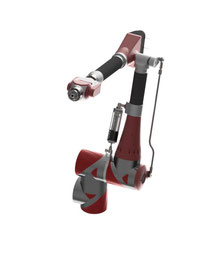
\includegraphics[width=0.6\textwidth]{arm.png}
\end{figure*}
\vspace{-1.8cm}

{\Huge\bf
PROJEKTSKIZZE: Lernen in Handarbeit
}
\\[2em]
\Large
{\bf Antragsteller:} Prof. Dr. Alexander Gepperth (HDR)\\
{\bf Adresse: } Fachbereich Angewandte Informatik der HAW Fulda\\
Leipzigerstr. 123, 36037 Fulda\\
{\bf Email: } alexander.gepperth@cs.hs-fulda.de\\
{\bf Telefon: } 0661 9640 3485\\
\vspace{0.5cm}

{\bf Projektdauer:} 9 Monate\\
\vspace{0.5cm}

{\bf Gesamtkosten:} 150.000\euro\\
\vspace{0.5cm}

{\bf Zuwendungsbedarf:} 150.000\euro\\
\vspace{0.5cm}

%{\bf Konsortium:} Assisted Living, Hilfe für Schwerbehinderte, Service-Robotik, 3D-Simulation
\end{center}
%\end{titlepage}
\newpage

\renewcommand{\thesection}{2}
\section{Antragsteller und assoziierte Partner}
Projektleiter des Projektes ist Herr Prof. Dr. Alexander Gepperth. Prof. Gepperth hat Kompetenzen/Erfahrung/Projekte etc...

\renewcommand{\thesection}{3}
\section{Ausgangsfrage und Ziele des geplanten Vorhabens}

\begin{itemize}
	\item Ziel: Demonstratorsystems zur Visualisierung der Funktionsweise des überwachten Lernens mittels NN
	\item Aufbau eines Handgestenerfassungs + Croppingsystems
	\item Einspeisung + Visualisierung der erfassten Daten für die Benutzer
	\item Visualisierung der Klassifikationsgüte (schlecht - mittel - gut)
	\item Darstellung der Dateneinspeisung, des Trainings, der Veränderung des Netzes + der Verbesserung der Klassifikationsgüte: Lernen durch Beispiele
	\item Deep Dreaming
	\item Handposen vs. Handgesten
	\item Forschungsaspekt: Inkrementelles Lernen

\end{itemize}


\subsection{Kurzzusammenfassung}
Das Projekt hat zum Ziel, ein interaktives Demonstrationssystem zur Veranschaulichung der Arbeitsweise maschinellen Lernens zu erstellen. 
Gegenstand des Lernens sind Handposen, die dem integrierten maschinellen Lernverfahren interaktiv durch direkte Demonstration vermittelt werden, bzw. welche das System nach
erfolgter Demonstration erkennt.  Hierbei wird nach jeder Erkennung der interne Zustand des Lernverfahrens, welcher zu einer Entscheidung geführt hat, visualisiert. 
Die hauptsächlichen Erkenntnisse zum maschinellen Lernen, die vermittelt werden sollen, lauten wie folgt: zunächst soll klargemacht werden, dass maschinelles Lernen alles andere als unfehlbar ist, vor allem dann, wenn Anzahl und Qualität der Daten unzureichend sind. Weiterhin soll durch eine detaillierte Visualisierung des internen Zustands des Lernverfahrens dargestellt werden, dass die grundsätzliche Arbeitsweise solcher Lernverfahren keine "schwarze Magie" darstellt, sondern auf anschaulicher Ebene  verstanden werden kann. 
Zu guter Letzt soll mit den im Laufe der Demonstration trainierten Handposen eine Applikation oder ein Spiel gesteuert werden, um die Praxisrelevanz zu verdeutlichen und zu transportieren, dass maschinelles Lernen auch großes Potential für Unterhaltung und Amüsement bietet. 
%
\subsection{Grundsätzliche Zielsetzung}
%
Maschinelles Lernen wird in er populären Wahrnehmung vielmals als mathematisch komplex und für Laien unverständlich wahrgenommen. Da maschinelle Lernverfahren in zunehmender Weise über Aspekte unseres täglichen Lebens entscheiden (z.B. bei der Kreditvergabe), führt diese Intransparenz nach unserer Auffassung dazu, das Misstrauen gegenüber maschinellen Lernverfahren zu erhöhen. Dem kann entgegengewirkt werden, indem gerade jungen MEnschen vermittelt wird, dass
die grundsätzliche Funktionsweise solcher Verfahren einfach nachzuvollziehen ist, sowie dass die Fähigkeiten von Lernverfahren fast ausschließlich von den Daten abhängen, mit denen sie trainiert werden. Das Ziel soll sein, dass maschinelle Lernverfahren als das gesehen werden was sie sind: als Werkzeuge, deren Funktionsweise man verstehen kann, statt als intransparente Entscheider. 
Das wird erreicht, indem Benutzergruppen in die Lage versetzt werden, ihr "eigenes" Lernverfahren durch direkte Demonstration zu trainieren, wobei live visualisiert wird, {\it warum} ein Verfahren zu einer bestimmten Entscheidung kommt.
%
\renewcommand{\thesection}{4}
\section{Ausführliche Vorhabensbeschreibung}\label{sec:besch}
\subsection{Einsatzszenario}
An der HAW Fulda existieren multiple Formate des Austauschs mit lokalen Schulen und der interessierten Öffentlichkeit: MINTMachClub\footnote{mint},Kinder-Universität\footnote{ku}, MINT-Labortage\footnote{mlt} sowie
reguläre Besuche von Schulklassen, oft aus der gymnasialen Oberstufe zur Hinführung auf ein mögliches Studium. Generell ist maschinelles Lernen für diese Zielgruppen sehr interessant und dessen Sinnhaftigkeit leicht vermittelbar, weswegen sich Präsentationen bzw- Demonstrationen für diese Zielgruppen oft überschneiden und wiederholen, was ein standardisiertes Format sinnvoll macht. 
Weiterhin ist allen Zielgruppen gemein, dass sie eher durch interaktive Lehrformate angesprochen und begeistert werden können, speziell in den niedrigeren Klassen. Hierbei macht es sicherlich Sinn, die Demonstration flexibel gestalten zu können:
rein interaktiv und relativ kurz für Schüler*innen ohne Informatik-Erfahrung, oder per API programmierbar für Oberstufenklassen im Rah,en eines Vormittagsprojekts. 
%
\subsection {Ablauf einer Demonstration}
Als Zielgruppe einer Demonstration wird eine Gruppe von 10 Personen oder mehr angenommen. Der erste Abschnitt besteht aus der gemeinsamen Definition der 
zu benutzenden Handposen. In der zweiten Phase demonstrieren bis zu 10 Personen gleichzeitig, auf Aufforderung des Demonstrators, einzelne Handposen, welche von Demonstrator registriert 
und zum Training der maschinellen Lernverfahrens genutzt werden. In der folgenden dritten Phase demonstrieren einzelne PErsonen Handposen, für welche der Demonstrator seine Klassifikationen ausgibt und
ausführlich visualisiert (Einzelkonfidenzen, Gesamtkonfidenz), wie diese Entscheidung zustande gekommen ist. Phasen 2 und 3 können beliebig oft wiederholt und der LErnfortschritt verglichen werden. Durch die Wiederherstellung vergangener Zustände und systematische Manipulation der gezeigten Handposen können verschiedene typische Effekte für fortgeschrittene Zielgruppen gezielt demonstriert werden, vor allem Overfitting und Generalisierung. 
%
Als letzte Demonstrationsphase sollen die Teilnehmer die dem System antrainierten Handposen nutzen, um eine Anwendung zu kontrollieren, wobei sich
die Steuerung eines Spiels bzw die Steuerung eines autonomen Roboters anbieten. Auch eine zur Verfügung Stellung der erkannten Handposen per ReST API ist denkbar, 
wobei dann die Reaktion eines Computersystems auf eine bestimmte Handpose von fortgeschrittenen Teilnehmern im Rahmen einer Projetkarbeitsphase selbst programmiert werden kann.
%
% TODO lernen der einschränkungen: linek hand trainieren, rechte testen --> problem!
\subsection{Technische Bausteine der Demonstration}
Für die Umsetzung des Demonstrators wird auf Techniken zurückgegriffen, welche bereits im Rahmen mehrerer Publikationen im Rahmen der Handposen- und Handgesterkennung implementiert und erprobt wurden \cite{gr1,gr2,gr3}, siehe auch Kap. \ref{sec:eigen}. Hierbei ist im Besonderen die Verarbeitung von 3D-Sensordaten, deren Transformation in kompakte aber aussagekräftige Beschreibungen (Deskriptoren) sowie die praxisorientierte Anwendung maschineller Lernverfahren, insbesondere neuronale Netze und DNNs. Die Implementierung kann auf einem einzelnen, allerdings leistungsfähigen Rechner mit High-End Grafikkarte statffinden, so dass sowohl die Sensordatenakquisition als auch deren Transformation in Deskriptoren sowie die Ausführung neuronaler Klassifkatoren mindestens 5 mal pro Sekunde erfolgen kann, idealweise öfter. Die Steuerung und Konfiguration der einzelnen Phasen des Demonstrators soll durch ein einfaches Sprachinterface erfolgen.
%
\section{Darstellung des Eigenanteils}\label{sec:eigen}
Die HAW Fulda hat tiefgehende Kompetenzen im Bereich des Maschinellen Lernens und modernen Interaktionstechniken. Im Bereich der modernen Interaktionstechniken (insb. Freihandgesten) wurde in bilateralen Forschungsvorhaben bereits ein Demonstrator zur Erkennung von Handgesten mittels 3D-Sensorik entwickelt (welcher hier mit geringfügigen Änderungen wieder zum Einsatz kommen soll). Mit Hilfe dieses Demonstrators konnten zahlreiche Erkenntnisse im Bereich des überwachten Lernens, der Sensordatenfusion und der Messung der kognitiven Last im Strassenverkehr gewonnen werden. So wurde in einem kooperativen Forschungsvorhaben nachgewiesen, dass die tatsächliche Ablenkung im Strassenverkehr während der Benutzung von Freihandgesten zur Steuerung von Infotainmentsystemen geringer ist als während der Bedienung durch Touchgesten oder Verwendung analoger Schaltelemente \cite{kopinski2016touch}. 
%
\begin{figure}[ht]
	\centering
  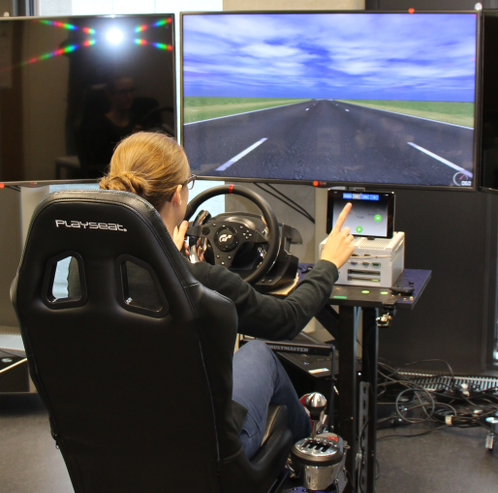
\includegraphics[width=0.7\textwidth]{images/simulator.png}
	\caption{Simulator}
	\label{fig1}
\end{figure}
%
Hierfür wurde der Demonstrator mit einem Strassenverkehrssimulator gekoppelt und somit konnten realistische Test mittels genormter Messanalysen durchgeführt werden. Aufbauend auf dem Demonstator wurden darüber hinaus zahlreiche Forschungsergebnisse im Bereich der 3D Sensordatenfusion und der mehrstufigen Klassifikation erzielt und veröffentlicht. So waren grundlegende Erkenntnisse, dass Daten aus Time-of-Flight Kameras sowohl früh als auch spät fusionieren um eine Verbesserung der Erkennungsrate zu erzielen \ref{kopinskineural}. Dieses ist insbesondere dahingehend interessant, da es unterschiedliche Performancegewinne des Systems nach sich zieht, was insbesondere für Handgestenerkennung in Echtzeit von hoher Praxisrelevanz ist. Darüber hinaus wurde mit Hilfe von mehrstufigen Neuronalen Netzen nachgewiesen, dass man Informationen aus bereits trainierten Netzen verwenden kann, um eine verbesserte Gesamtperformance des Systems zu erreichen, indem man die Erkennungsgüte mit vortrainierten Netzen stabilisiert \ref{kopinski2015pragmatic}. Diese Erkenntnisse bildeten die Grundlage für die Erkennung von Handposen und die Erkennung von dynamischen Handgesten auf Basis stabiler Posen \ref{kopinski2015real}. Letztlich wurde durch den Einsatz von Deep Learning Verfahren ein eigener Ansatz entwickelt, mittels dessen Erkenntnisse aus dem Bereich der 2D-Bilderkennung in den 3D-Raum übertragen werden konnten \ref{kopinski2016deep}.  
%
% TODO: Daten von mehreren Personen!
% TODO: Zitate!
\renewcommand{\thesection}{6}
\section{Nachhaltigkeit,Übertragbarkeit}
\textbf {Forschungsprojekte} Der Antragsteller hat umfangreiche Vorarbeiten im Bereich des maschinellen Lernens erbracht, vor allem im Bereich der Handposen- und Gestenerkennung, der Objekterkennung sowie des inkrementellen Lernens mit neuronalen Netzen (DNNs). 
Ein implementierter Demonstrator so wie er in Kap. \ref{sec:besch} beschreiben ist, könnte für weiter gehende Forschungsprojekte und Forschungsanträge des Antragstellers von großem Nutzen sein, hauptsächlich aufgrund der Fähigkeit, Handposen und Handgesten von mehreren Personen gleichzeitig aufzunehmen. Dies kann die Akquisition eine großen Menge qualitativ hochwertiger Trainingsdaten, deren Gewinnung ja stets das Hauptproblem eines jeden Projekts im Bereich des maschinellen Lernens darstellt, stark vereinfachen. Des Weiteren kann der Demonstrator auch dazu dienen, methodische Fortschritte einfach zu verdeutlichen (z.B. als zusätzliche Ressourcen beim Einreichen eines Konferenzbeitrags oder als Live-Demo während eines Vortrags). Hierbei ist im Besonderen an die Arbeiten des Antragstellers zum inkrementellen Lernen zu denken, welche untersuchen, wie DNNs neue Kenntnisse dazulernen können \cite{xx}. Anhand des Demonstrators lässt sich die Tatsache, dass ein Lernverfahren eine neue, soeben demonstrierte Handpose erfolgreich dazugelernt und die bereits vorher beherrschten nicht vergessen hat, lässt sich einfach und anschaulich demonstrieren.

\textbf{Lehre}
Der Antragsteller ist Modulverantwortlich für die Module "Künstliche Intelligenz" und "Machine Learning" auf Bachelor-bzw. Master-Niveau. Vor allem auf Bachelor-Niveau wo die mathematischen Grundlagen des maschinellen Lernens noch nicht vertieft eingeführt werden können, wird es ein Demonstrator für Handposenerkennung ermöglichen, auch konzeptuell abstrakte Ideen wie z.B. Overfitting, Underfitting, Sampling Bias oder Generalisierung anschaulich zu erläutern. Selbstverständlich können auch die vom Demonstrator aufgenommenen Daten auch für kleine Projekte im Rahmen der Lehrveranstaltungen eingesetzt werden. Auch ein Einsatz im Bereich der Vorlesung "Robotik" ist sinnvoll, in welcher evtl. eine Handposensteuerung für autonome Roboter als Projekte umgesetzt werden kann.
%
\renewcommand{\thesection}{7}
\section{Zeitplan}
\begin{itemize}
\item Projektmanagement Maerz-Dez
\item Aufbau des Systems: Maerz - August
\item Exkursion + Workshop: September - Dezember

\end{itemize}

\renewcommand{\thesection}{8}
\section{Finanzierungsplan}
Es werden die folgenden Kostenpunkte zur Durchführung de Projekts angesetzt. Jeder Punkt wird einzeln im Hinblick auf seine Notwendigkeit und Verhältnismäßigkeit 
diskutiert und begründet. Generell wird davon ausgegangen, dass 4 Demonstratoren gleichzeitig ausgerüstet werfen, um bei "parallelen" Veranstaltungen jeder Gruppe eine Demonstration zeigen zu können. Dies ist bei Projekten, wo viele Schüler an einem oder zwei Tagen ein Projektprogramm absolvieren, relativ häufig der Fall und begründet diese Grundsatzentscheidung.
\begin{itemize}
%50\% Stelle Data Science E11 - TVL 11: 27.058,19
\item \textbf{1 Wissenschaftliche Mitarbeiter*in E11 - TVL 11/2 (27.058,19\euro)} Diese Mitarbeiter*in soll die Demonstrator-Plattform unter Anleitung des Antragstellers und unter Einbeziehung bereits existierenden Programmcodes implementieren. Gesucht wird eine Person mit stark ausgeprägten Programmierfähigkeiten und Erfahrung in der Sensordatenverbeitung. Da 
zur Implementierung des Demonstrator-Plattform hauptsächlich bereits beschriebene System umgesetzt werden sollen, sind außer Grundkenntnissen keine speziellen Kenntnisse des maschinellen Lernens nötig, was die Suche nach geeigneten Kandidaten deutlich erleichtern sollte.
\item \textbf{Sensoren: 2000\euro} Hier ist die Beschaffung von ca. 6-8 3D-Sensoren (2 für jeden der 4 Demonstratoren) geplant. Diese Sensoren sollten bei Sonneneinstrahlung robust funktioneren, was reine Structured-Light-Ansätze ausschließt. Deshalb sind Hybridlösungen (Stereo + Structured Light) empfehlenswert, wie sie gegenwärtig für ca. 200\euro/Stück verfügbar sind.
\item \textbf{Rechner (10000\euro)} Es werden 4 möglichst identische Rechner plus eine Arbeitsplatzrechner benötigt. Ausstattung muss ein starkes Netzteil beinhalten (um die Grafikkarte zu versorgen), sowie neben einer leistungsfähigen Grafikkarte für das Training der maschinellen Lernverfahren ebenfalls über ausreichend Speicher verfügen muss. 
\item \textbf{Deputatsermässigung Abtragsteller 2SWS 1 Jahr (2000\euro)} Dies ist erforderlich, um in ausreichendem Maße an der Projektarbeit teilnehmen zu können, insbesondere um die Projektmitarbeiter*in anzuleiten.
\item \textbf{2 studentische Hilfskräfte für jeweils 6 Monate, 20h/Woche (8000\euro)} Notwendig für funktionale Tests des Demonstrators, Bugfixing sowie um Aspekte der Usability zu verifizieren. Ebenso zum Aufbau des Demonstrators und zur Durchführung von Demonstrationen.
\end{itemize}


%\renewcommand{\refname}{}
\bibliographystyle{abbrv}
\bibliography{bib}
%

\end{document}




